\documentclass{beamer}
\usepackage{times}
\usepackage[czech]{babel}
\usepackage[utf8]{inputenc}
%\usetheme{Berkeley}
%\usetheme{Copenhagen}
\usetheme{Madrid}
%\usecolortheme{beaver}
\newcommand{\czuv}[1]{\quotedblbase #1\textquotedblleft}
\usepackage{graphicx}
\setbeamertemplate{caption}[numbered]
\usepackage{fancyvrb}
%\nonstopmode

\newcommand\br[1]{\textcolor{red}{\textbf{#1}}}
\title[Prezentace k předmětu Semestrální projekt]{Rozšíření systému pro získávání, zpracování a~analýzu rozsáhlých kolekcí textů z webu}
\author{Matějka Jiří}
\date{31. 1. 2018}
\logo{
\includegraphics[width=4.5cm]{fit.png}}

\begin{document}
  \frame{\titlepage}
%%%%%%%%%%%%%%%%%%%%%%%%%%%%%%%%%%%%%%%%%%%%
  \begin{frame}
    \frametitle{Motivace}
	Dosavadní systém:
	\begin{itemize}
		\item \br{jednorázové} vytvoření korpusu z \br{předem shromážděných} dat (zatím ověřeno pouze na angličtině)
	\end{itemize}
	Omezení:
	\begin{itemize}
		\item jednotlivé kroky zpracování korpusových dat vyžadují \br{ruční zásahy}
		\item nejsou ošetřeny chybové stavy prvotních fází zpracování
		\item není možné korpusová data a indexy snadno aktualizovat
		\item nelze odhadnout, jak dlouho bude zpracování nových dat probíhat
	\end{itemize}
	% Odkud brát nová data:
	% \begin{itemize}
	% 	\item Atom a RSS zdroje,
	% 	\item blogy,
	% 	\item komentáře u článků,
	% 	\item sociální sítě,
	% 	\item ...
	% \end{itemize}
  \end{frame}
%%%%%%%%%%%%%%%%%%%%%%%%%%%%%%%%%%%%%%%%%%%%
  \begin{frame}
    \frametitle{Zpracování}
	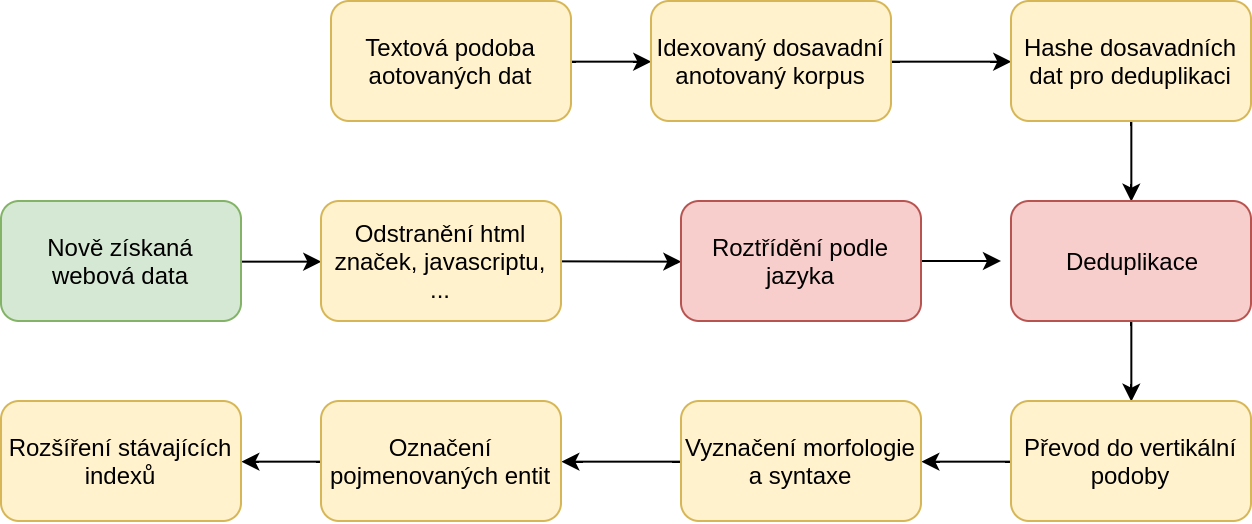
\includegraphics[width=\linewidth]{pipeline.png}
  \end{frame}

%%%%%%%%%%%%%%%%%%%%%%%%%%%%%%%%%%%%%%%%%%%%%%%%%%%
  \begin{frame}
    \frametitle{Práce v 1. semestru a zjištěné problémy}
	Práce během semestru:
	\begin{itemize}
		\item \br{dokončení prototypu} a jeho spuštění nad reálnými daty
		\item tvorba a testování nových skriptů pro kolekci a stahování dat
	\end{itemize}
	Zkušební spuštění (100 souborů, 22 GiB dat):
	\begin{itemize}
		\item Povedlo zpracovat bezchybně 74 souborů
		\item 7 souborů skončilo s \br{chybou během vertikalizace}
		\item u 19 souborů se objevily \br{chyby behěm formátování dat} pro morfologické značení a syntakcké značení
	\end{itemize}
	Problémy:
	\begin{itemize}
		\item spousta logů, u chyb často není možné zjitit přesnou příčinu
		\item spousta skriptů (často i nečitelných)
%		\item vertikalizace není úplně vychytaná (např. neošetřené chybové stavy)
		\item zpracování není automatizované
	\end{itemize}
  \end{frame}

 %%%%%%%%%%%%%%%%%%%%%%%%%%%%%%%%%%%%%%%%%%%%%%%%%%
  \begin{frame}
    \frametitle{Časový plán na 2. semestr}
	\begin{itemize}
		\item \br{sjednocení skriptů} do větších celků (použití přepínačů, sdílené moduly) -- během února
		\item podrobně \br{analyzovat vertikalizátor} a buď \br{opravit chyby} nebo \br{najít vhodnější řešení} -- během března (možná i duben)
		\item zautomatizovat zpracování a umožnit aktualizaci dat -- duben
		\item sledování zpracování, \br{měření náročnosti na procesor a paměť}, tvorba statistik -- duben, květen
	\end{itemize}
	Během tvorby veškerých skriptů bude dbán důraz na:
	\begin{itemize}
	  \item snadno parsovatelné logy regulárnímy výrazy nebo skripty
	  \item vedení podrobných statistik už během zpracování, možnost zasílat statistická data i chybová hlášení emailem
	\end{itemize}
  \end{frame}
  %%%%%%%%%%%%%%%%%%%%%%%%%%%%%%%%%%%%%%%%%%%%%%%%%%


\end{document}
